\chapter{Memory Model}
We will now beging to expand on some of the block is \autoref{fig:prog_mod_v0}. Before starting to explore how the CPU works, it's useful to have an understanding of how memory is laid out. We will start looking at the flash and RAM blocks. Together with another block called perihperals (which we will explore later), these blocks make up memory. 
It's important to note that this memory is located \emph{outside} of the CPU, but still inside the microcontroller IC.

The memory of a device can be though of as a very long row of post boxes along a street. 
Each post box has an address, and each post box can have data put into it or taken out. The amount of data that each post box can hold is 8 bits, or one byte. Therefore, each memory address is said to address one byte. 
The address of each post box is 32 bits long, meaning that addresses range from 0 (0x00000000) to just over 4.3 billion (0xFFFFFFFF). In actual fact, the \emph{vast} majority of these addresses do not have a post box at them. These addresses are said to be unimplemented. 
Only very small sections of this address space are implemented and can actually be read from or written to.
Flash and RAM are contiguous blocks of memory, with a start address and an end address. A simplified memory map of the STM32F051 is shown in \autoref{fig:memory_map}. From this, we can see that if we want to use changeable variables in our programs, the variables should be located at addresses between 0x2000 0000 and 0x2000 1FFF. If we want to load code onto the micro which should not be lost when the device loses power, the code should be loaded into the non-volatile memory, flash, which has addresses between 0x0800 0000 and 0x0800 7FFF.
If we want the ability to modify data during the execution of our program, the data should be placed in the read/write section of memory, RAM. 

\begin{figure}
  \centering
  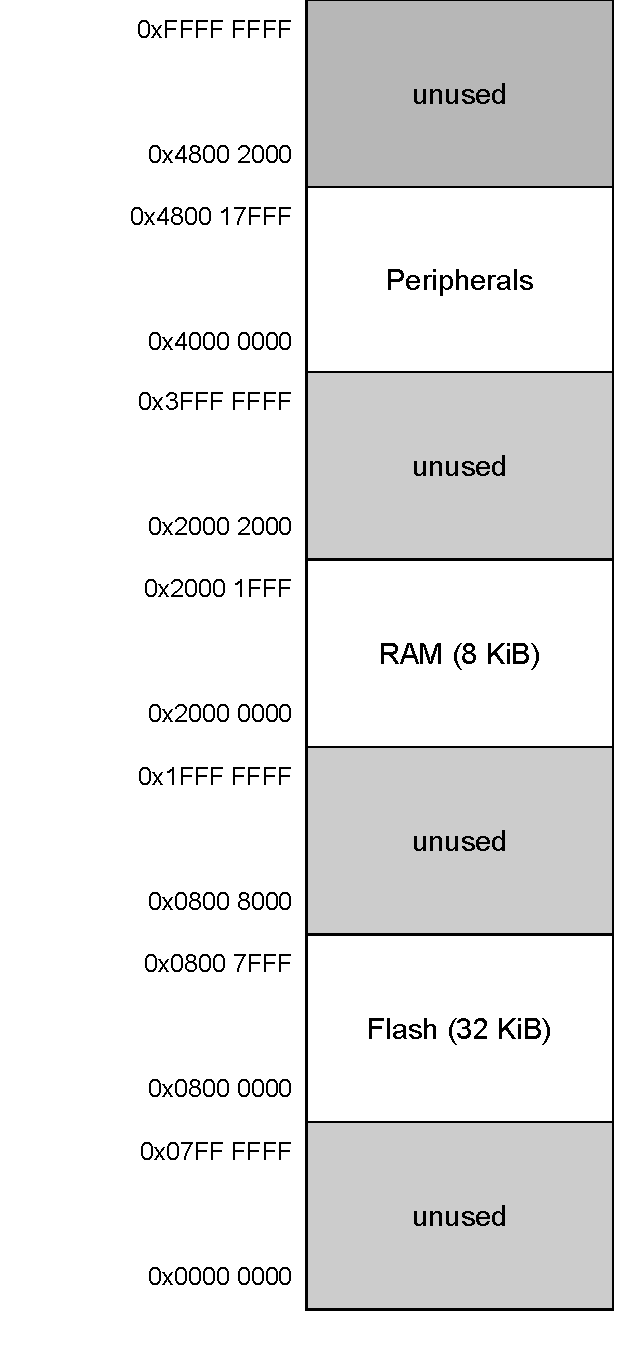
\includegraphics[width=0.6\textwidth]{./week1/memory_model_v0.pdf}
  \caption{Simplified STM32F051C6 memory map. Note how all addresses are 32 bits. The blocks are very much not to scale. Source: datasheet, Figure 9}
  \label{fig:memory_map}
\end{figure}

\section{Data Types and Endianness}
Very often we will need to work with clumps of data which are larger than 1 byte. ARM defines datatypes for a 32 bit CPU as follows:
\begin{itemize}
  \item byte: 8 bits
  \item halfword: 16 bits
  \item word: 32 bits
  \item doubleword: 64 bits
\end{itemize}
Each memory address only addresses one byte of memory, so how can something like a word (four bytes) be stored in memory? 
Obviously, the four bytes have to come after each other to form a four byte block, or word.
However, it is not obvious which order they should come in. For example, consider the case of wanting to store the word 0xAABBCCDD in address 0. The two possible ways of doing it are shown in \autoref{tab:endianness}. It doesn't really matter which one of these schemes is used - they each have their pros and cons and different processors use different methods. It is important to know which one our processor has chosen to use. Our processor uses little endian. A more abstract view of how data is stored in our processor is given in \autoref{fig:little_end_prog_man}
\newpage
\begin{table}
\centering
\begin{tabu}{cc}
    \multicolumn{2}{c}{\textbf{Little Endian}}\\
    \hline
    Address & Data \\
      \hline
      3 & 0xAA \\
      2 & 0xBB \\
      1 & 0xCC \\
      0 & 0xDD \\
\end{tabu}
\qquad
\begin{tabu}{cc}
    \multicolumn{2}{c}{\textbf{Big Endian}}\\
    \hline
    Address & Data \\
      \hline
      3 & 0xDD \\
      2 & 0xCC \\
      1 & 0xBB \\
      0 & 0xAA \\
\end{tabu}
\caption{Layouts of the word 0xAABBCCDD in memory at effective address 0, according to little or big endian format}
\label{tab:endianness}
\end{table}

\begin{figure}
  \centering
  \includegraphics[width=0.8\textwidth, page=21, clip=true, trim=160px 285px 160px 427px]{./stm32f0xx_programming_manual.pdf} % l b r t
  \caption{More abstract view of little endian layout. Source: Prog Man, page 28}
  \label{fig:little_end_prog_man}
\end{figure}

%\begin{overpic}[page=21, grid,unit=1px, tics=20, clip=true, trim=160px 285px 160px 427px]{./stm32f0xx_programming_manual.pdf}
%\end{overpic}

